% Template LaTeX document for CSSR4Africa Deliverables
% Adapted from documents prepared by EPFL for the RobotCub project
% and subsequently by the University of Skövde for the DREAM project
%
% DV 28/06/2023

\documentclass{CSSRforAfrica}

\usepackage{array}
\usepackage{caption}
\usepackage{dirtree}
\usepackage{float}
\usepackage{fontenc}
\usepackage{geometry}
\usepackage{graphicx}
\usepackage{latexsym}
\usepackage{listings}
\usepackage{lmodern}
\usepackage{longtable}
\usepackage{pdflscape}
\usepackage{pdfpages}
\usepackage[table,dvipsnames,svgnames]{xcolor}
\usepackage{tikz}
\usepackage[titletoc,title]{appendix}
\usepackage{url}
\usepackage{tabularx,colortbl}
\usepackage{verbatim}
\usepackage{subcaption}
\usepackage{multicol}
\usepackage[hidelinks,colorlinks=false]{hyperref}
\usetikzlibrary{shapes.geometric, positioning, arrows.meta,shapes,arrows, calc}
\captionsetup[figure]{format=hang}
\definecolor{backcolour}{rgb}{0.95,0.95,0.95} 
\definecolor{codegreen}{rgb}{0,0.6,0}
\definecolor{codepurple}{rgb}{0.5,0.0,0.5}
\definecolor{greenyellow}{rgb}{0.8, 0.7, 0.10}

\lstdefinestyle{withoutNumbering}{
    backgroundcolor=\color{backcolour},   
    commentstyle=\color{codegreen},
    keywordstyle=\color{magenta},
    stringstyle=\color{codepurple},
    %%basicstyle=\ttfamily\small,
    basicstyle=\ttfamily\scriptsize,
    breakatwhitespace=false,         
    breaklines=true,                 
    captionpos=b,                    
    keepspaces=true,                 
    showspaces=false,                
    showstringspaces=false,
    showtabs=false,                  
    tabsize=2
}

% Define custom colors
\definecolor{backcolour}{rgb}{0.95,0.95,0.92}
\definecolor{codegreen}{rgb}{0,0.6,0}
\definecolor{codeblue}{rgb}{0,0,0.8}
\definecolor{codepurple}{rgb}{0.58,0,0.82}
\definecolor{darkred}{rgb}{0.6,0,0.0}
\definecolor{brown}{rgb}{0.6,0.4,0.2}

% Define a custom XML language with keywords for different node types
\lstdefinelanguage{XMLCustom}{
    morestring=[b]",
    morestring=[b]',
    morecomment=[s]{<!--}{-->},
    sensitive=true,
    % Control Flow Nodes:
    morekeywords={
      Sequence, Fallback, Parallel, Inverter, RetryUntilSuccessful, KeepRunningUntilFailure, ForceFailure
    },
    % Tree Nodes:
    alsoletter={<},
    morekeywords=[2]{
      root, BehaviorTree, SubTree, START_OF_TREE
    },
}

% Define the style for XML code
\lstdefinestyle{XMLStyle}{
    language=XMLCustom,
    backgroundcolor=\color{backcolour},
    basicstyle=\ttfamily\small,
    %%basicstyle=\ttfamily\footnotesize,
    commentstyle=\color{codegreen},
    keywordstyle=\color{codeblue}\bfseries,
    keywordstyle=[2]\color{brown}\bfseries,
    stringstyle=\color{codepurple},
    breaklines=true,
    breakatwhitespace=true,
    showstringspaces=false,
    captionpos=b,
    escapeinside={(*@}{@*)},
    literate={<}{{\textcolor{darkred}{<}}}1 {>}{{\textcolor{darkred}{>}}}1 {</}{{\textcolor{darkred}{</}}}2
}



\hypersetup{
    colorlinks=true,
    linkcolor=black,
    filecolor=magenta,      
    urlcolor=blue,
    citecolor=blue,
    pdfpagemode=FullScreen
    }



\newcommand{\blank}{~\\}
\newcommand{\checkbox}{{~~~~~~~\leavevmode \put(-7,-1.5){  \huge $\Box$  }}}


 
%% Directory Tree Font
%\renewcommand*\DTstyle{\rmfamily\footnotesize}
%\renewcommand*\DTstyle{\sffamily\footnotesize}
%\renewcommand{\DTstyle}{\small\ttfamily}
\renewcommand{\DTstyle}{\footnotesize \ttfamily}
%\renewcommand{\DTstyle}{\scriptsize \ttfamily}

\captionsetup[figure]{format=hang}

\begin{document}
\input{epsf}

%%
%% SHOULD NOT NEED TO BE CHANGED BEFORE THIS POINT
%% ------------------------------------------------
%%

\deliverable{D6.1}              
\title{6.1  Use Case Implementation}   

\leadpartner{Carnegie Mellon University Africa (for Wits)}      
\partner{Carnegie Mellon University Africa}                               

\revision{1.2}                           
\deliverabledate{31/03/2025}  
\submissiondate{18/04/2025}  
\revisiondate{01/06/2025}      
\disseminationlevel{PU}
\responsible{D. Vernon }       


%%
%% Create the titlepage
%%

\maketitle
 

\section*{Executive Summary}
%===============================================================
\label{executive_summary}
%%\addcontentsline{toc}{section}{Executive Summary}
 
Deliverable D6.1  documents the outcome of Task 6.1, i.e., the  implementation of the two  use cases defined in Work Package WP2, using the outcomes of WP1 - WP5, i.e., the cultural knowledge, the scenario specification, and the integrated  robot's sensory and interaction capabilities.
Specifically, the use cases are captured using the robot mission specification methodology documented in Deliverable D5.4.2 Robot Mission Language, i.e., using behavior trees \cite{Ghzoulietal2023,DortmansPunter2022}. The resultant behavior tree provides the input to the {\small \tt behaviorController} ROS node documented in Deliverable D5.4.3.  Running the {\small \tt cssr\_system} ROS package against the behavior tree robot mission specification provides a demonstration of the complete working system for the corresponding  use case. 

In the CSSR4Africa work plan, this deliverable is assigned to the University of the Witswatersrand. However, the material in this  report was developed and written by Carnegie Mellon University Africa. This was necessary because, due to extensive delays in the delivery of the Pepper robot to the University of the Witswatersrand, little or no progress had been made on three key inputs for Task 6.1 and Deliverable D6.1, viz. Deliverables D5.4.1 Cultural Knowledge Ontology \& Culture Knowledge Base, D5.4.2 Robot Mission Language, and D5.4.3 Robot Mission Interpreter, all of which were assigned to the University of the Witswatersrand.  Consequently,  Carnegie Mellon University Africa took joint responsibility for these four deliverables (among others, specificially D5.5.2.1, D5.5.4, D6.2). Since this involved a significant amout of additional, unplanned effort, only one use case, the laboratory tour,  has been implemented to date, leaving the second use case, the receptionist, to be implemented later.
  
\pagebreak
\tableofcontents
\newpage


\section{Introduction}
%===============================================================
 \label{section:introduction}

This deliverable provides a detailed walkthrough of the behaviour tree implementation  the Lab Tour robot mission specification, as defined by the D2.1 Use Case Scenario. Section \ref{section:xml_output}  introduces the generated XML output, which is the representation of robot mission specification behavior tree, by describing the organization of the XML file. Section \ref{section:subtrees} discusses the incorporation and structuring of subtrees, which modularize complex behaviors within the mission specification. For each subtree, corresponding XML definition and graphical illustration are provided. Additionally, Section \ref{section:mission_nodes} explains mission nodes, which represent specific tasks or actions executed by the robot.



 
\section{Behaviour Tree Implementation of Use Case Scenario 1: Laboratory Tour}
%===============================================================
\label{section:bt_implementation}

This section details the implementation of a robot mission specification based on the operational guidelines provided in the ``Lab Tour'' scenario (see Deliverable D2.1 User Scenario Specification). While the mission is grounded in the scenario described in D2.1, there are minor deviations from the original step-by-step narrative to accommodate implementation constraints and practical considerations. The mission is structured as a behavior tree, which serves as the control architecture for coordinating the robot’s actions. To design and visualize this behavior tree, we employ the Groot2 IDE, using its intuitive drag and drop mechanisms as outline above. The mission interpreter, implemented using the BehaviorTree.CPP library (described in Deliverable D5.4.3 Robot Mission Interpreter), executes the behavior tree within a ROS-based framework, forming an integral part of the CSSR4Africa software system. For an overview of the system architecture, please refer to D3.1 System Architecture.


\subsection{XML Output}
%--------------------
\label{section:xml_output}

As explained above, the mission is designed using the Groot2 IDE. The Groot2 IDE allows for the design of behavior trees using a graphical interface. The mission specification represented as a behavior tree is then exported as an XML file, which is used by the mission interpreter to execute the mission. 
The XML representation of the behavior tree designed for the ``Lab Tour'' scenario is explained in the following sections, along with the graphical illustrations for each segment of the behavior tree.

The robot mission specification file is has three sections, the file root, the subtree specifications, and the mission nodes. These are described in the following sections.

\newpage
\subsection{File Root}
%-----------------
\label{section:file_root}
The root element of the XML file is defined as:
\begin{lstlisting}[style=XMLStyle, language=XMLCustom]
    <?xml version="1.0" encoding="UTF-8"?>
    <root BTCPP_format="4" main_tree_to_execute="TourGuide">
    <!-- .... -->
    </root>
\end{lstlisting}
The attribute \texttt{BTCPP\_format="4"} specifies that this behavior tree is built for version 4 of the BehaviorTree.CPP library.
This is important because the robot mission interpreter must be implemented with the correct version, in this case, version 4, for the behavior tree specification to be executed correctly. It is worth noting that the Groot2 IDE supports both version 3 and version 4 of the library, configurable within the settings, so this attribute helps ensure compatibility between the designed behavior tree and the mission interpreter. The attribute \texttt{main\_tree\_to\_execute="TourGuide"} designates \texttt{TourGuide} as the primary behavior tree to be executed, indicating which tree within the file serves as the entry point for the mission.

 \vspace{-1mm}
\subsection{Subtrees}
% For each subtree follow a pattern of description, figure, and XML.
%-----------------
\label{section:subtrees}
 
To facilitate an efficient mission design process and enhance readability and clarity, the overall mission was structured into several distinct subtrees, each representing a logical segment of the overall task defined in the use case scenario. 
This enabled easier development and debugging and allows for future modifications. By organizing the behavior tree into modular, clearly defined subtrees, the complexity of mission specifications is significantly reduced. Then, by connecting these modular subtrees in a well-defined logical sequence, the final behavior tree is constructed, which serves as the complete mission specification for the use case scenario as defined in Deliverable D2.1 Use Case Scenario.
  
\vspace{-1mm}
\subsubsection{TourGuide Subtree}
%- - - - - - - - - - - - - - 
\vspace{-2mm}
The \texttt{TourGuide} subtree is the main behavior tree that orchestrates the robot's actions during the tour. It begins with the \texttt{StartOfTree} action node and is composed of five sequential subtrees, each representing a distinct phase of the tour interaction. The segments are executed sequentially, with the robot transitioning from one segment to the next based on the outcome of the previous segment.  The behavior tree diagram of the \texttt{TourGuide} subtree is shown in Figure \ref{fig:tourguide_diagram}. The XML representation of the TourGuide subtree is shown in Listing \ref{lst:tourguide_xml}.

% Tree diagram
\begin{figure}[H]
  \centering
  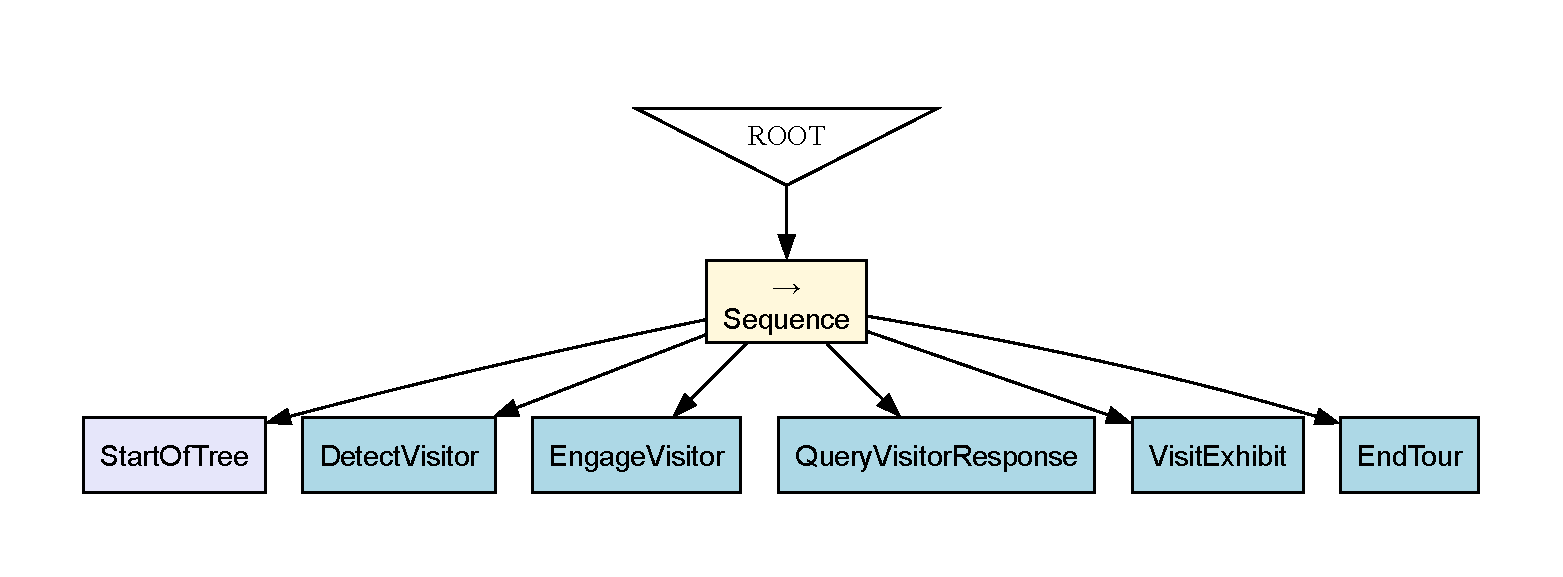
\includegraphics[width=\textwidth]{./diagrams/main.pdf}
  \caption{Behavior Tree Diagram of the ``TourGuide'' Subtree}
  \label{fig:tourguide_diagram}
\end{figure}

%XML representation
\begin{lstlisting}[
  style=XMLStyle, 
  language=XMLCustom, 
  caption={XML Representation of the ``TourGuide'' Subtree},
  label={lst:tourguide_xml}
]
<BehaviorTree ID="TourGuide">
  <Sequence>
    <StartOfTree/>
    <SubTree ID="DetectVisitor"/>
    <SubTree ID="EngageVisitor"/>
    <SubTree ID="QueryVisitorResponse"/>
    <SubTree ID="VisitExhibit"/>
    <SubTree ID="EndTour"/>
  </Sequence>
</BehaviorTree>
\end{lstlisting}


 
\subsubsection{DetectVisitor Subtree}
% %- - - - - - - - - - - - - - - - - - - - -} 

The DetectVisitor subtree is dedicated to identifying when a visitor is present. Before initiating visitor detection, however, the robot first retrieves the list of exhibits to be visited and initializes its own starting position within the environment. It then utilizes various sensors available to the robot to continuously monitor its surroundings. The robot is animated to appear lively, actively scanning its environment to reliably localize and track a visitor before initiating an interaction. 

% Tree diagram
\begin{landscape}
\hspace{3cm}
\vspace{3cm}
\begin{figure}[H]
  \centering
  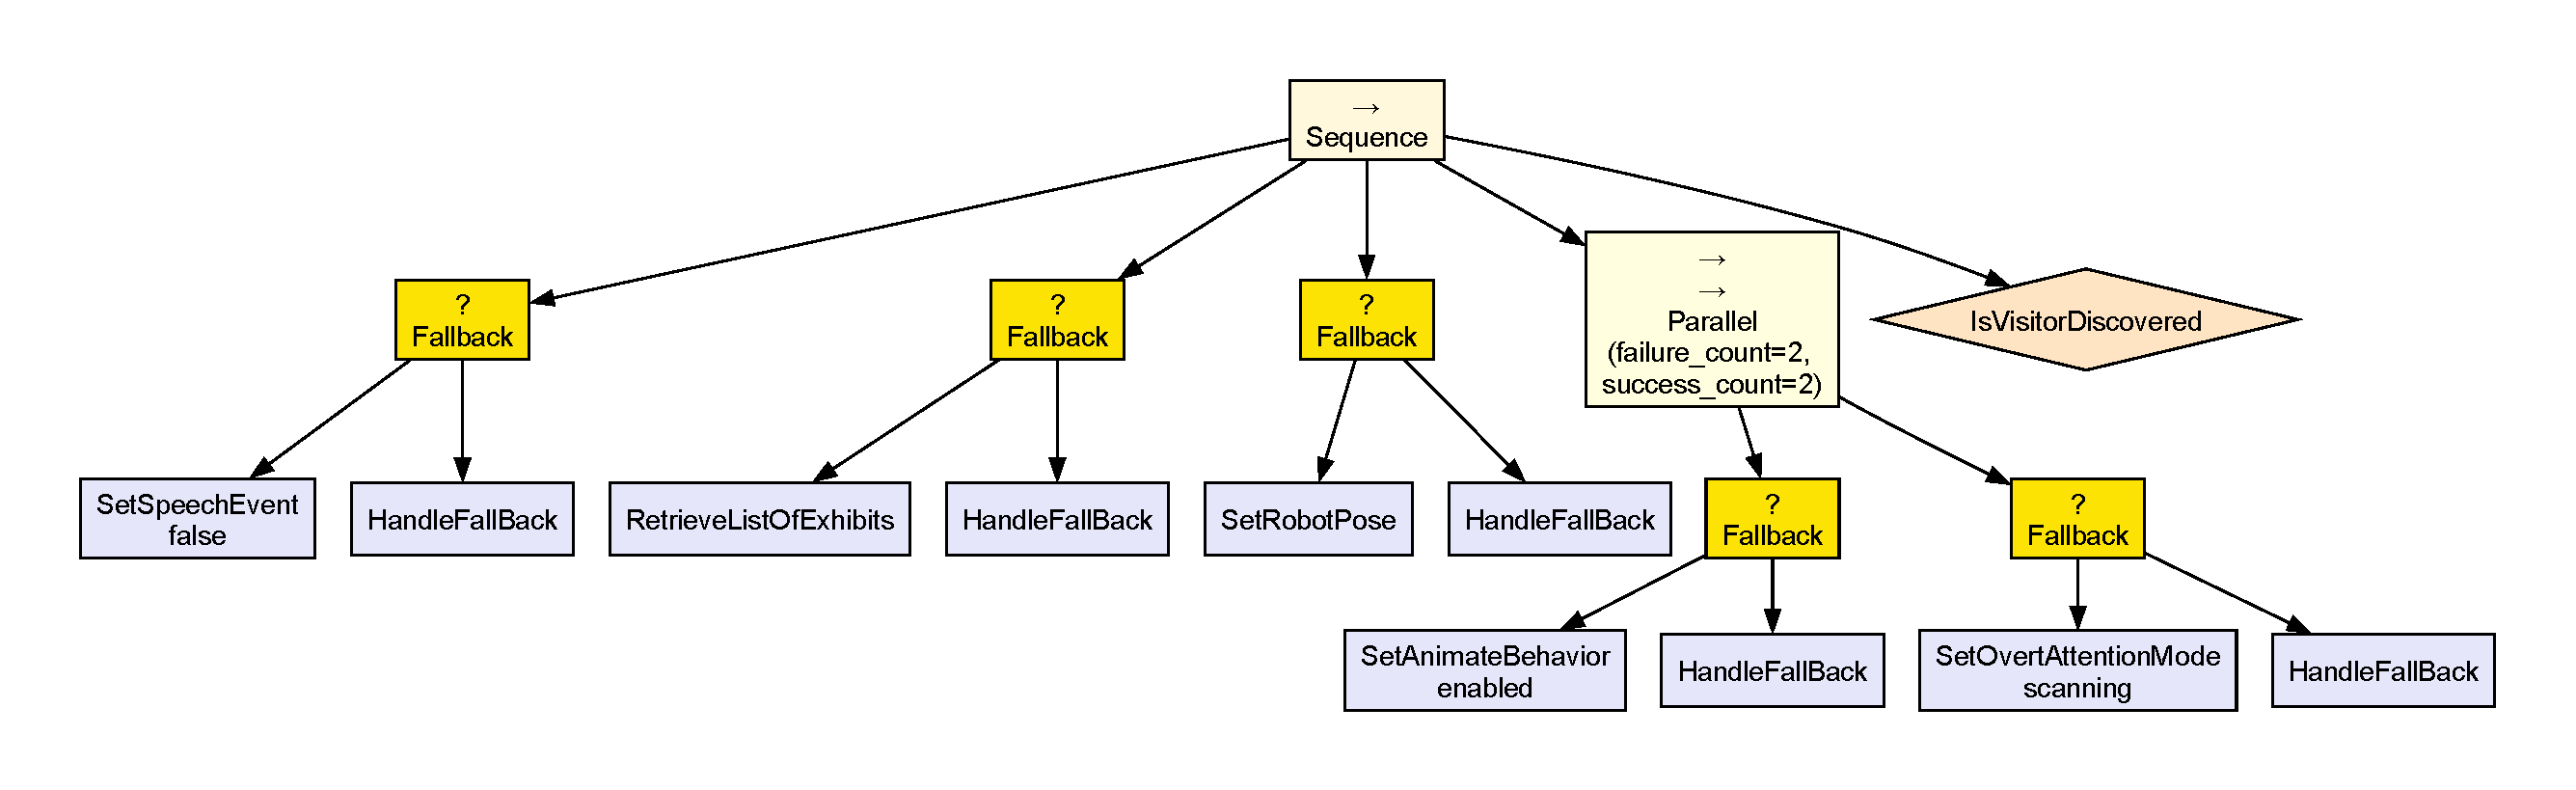
\includegraphics[width=1.55\textwidth]{./diagrams/detect.pdf}
  \caption{Behavior Tree Diagram of the ``DetectVisitor'' Subtree}
  \label{fig:detect_visitor_diagram}
\end{figure}
\end{landscape}

%XML representation
\begin{lstlisting}[
  style=XMLStyle, 
  language=XMLCustom, 
  caption={XML Representation of the ``DetectVisitor'' Subtree},
  label={lst:detect_visitor_xml}
]
<BehaviorTree ID="DetectVisitor">
    <Sequence>
      <Fallback>
        <SetSpeechEvent name="false"/>
        <HandleFallBack/>
      </Fallback>
      <Fallback>
        <RetrieveListOfExhibits/>
        <HandleFallBack/>
      </Fallback>
      <Fallback>
        <SetRobotPose/>
        <HandleFallBack/>
      </Fallback>
      <Fallback>
        <SetAnimateBehavior name="enabled"/>
        <HandleFallBack/>
      </Fallback>
      <Fallback>
        <SetOvertAttentionMode name="scanning"/>
        <HandleFallBack/>
      </Fallback>
      <IsVisitorDiscovered/>
    </Sequence>
  </BehaviorTree>
\end{lstlisting}


\subsubsection{EngageVisitor Subtree}
%- - - - - - - - - - - - - - - - - - - - -} 

Once a visitor is detected, the robot transitions to actively engaging them. In this phase, the robot makes a welcoming gesture, greets the visitor verbally, and introduces itself as the tour guide. The engagement involves adjusting its body language to establish a friendly and approachable interaction.
% Tree diagram
\begin{landscape}
\begin{figure}[H]
  \vspace{3cm}
  \centering
  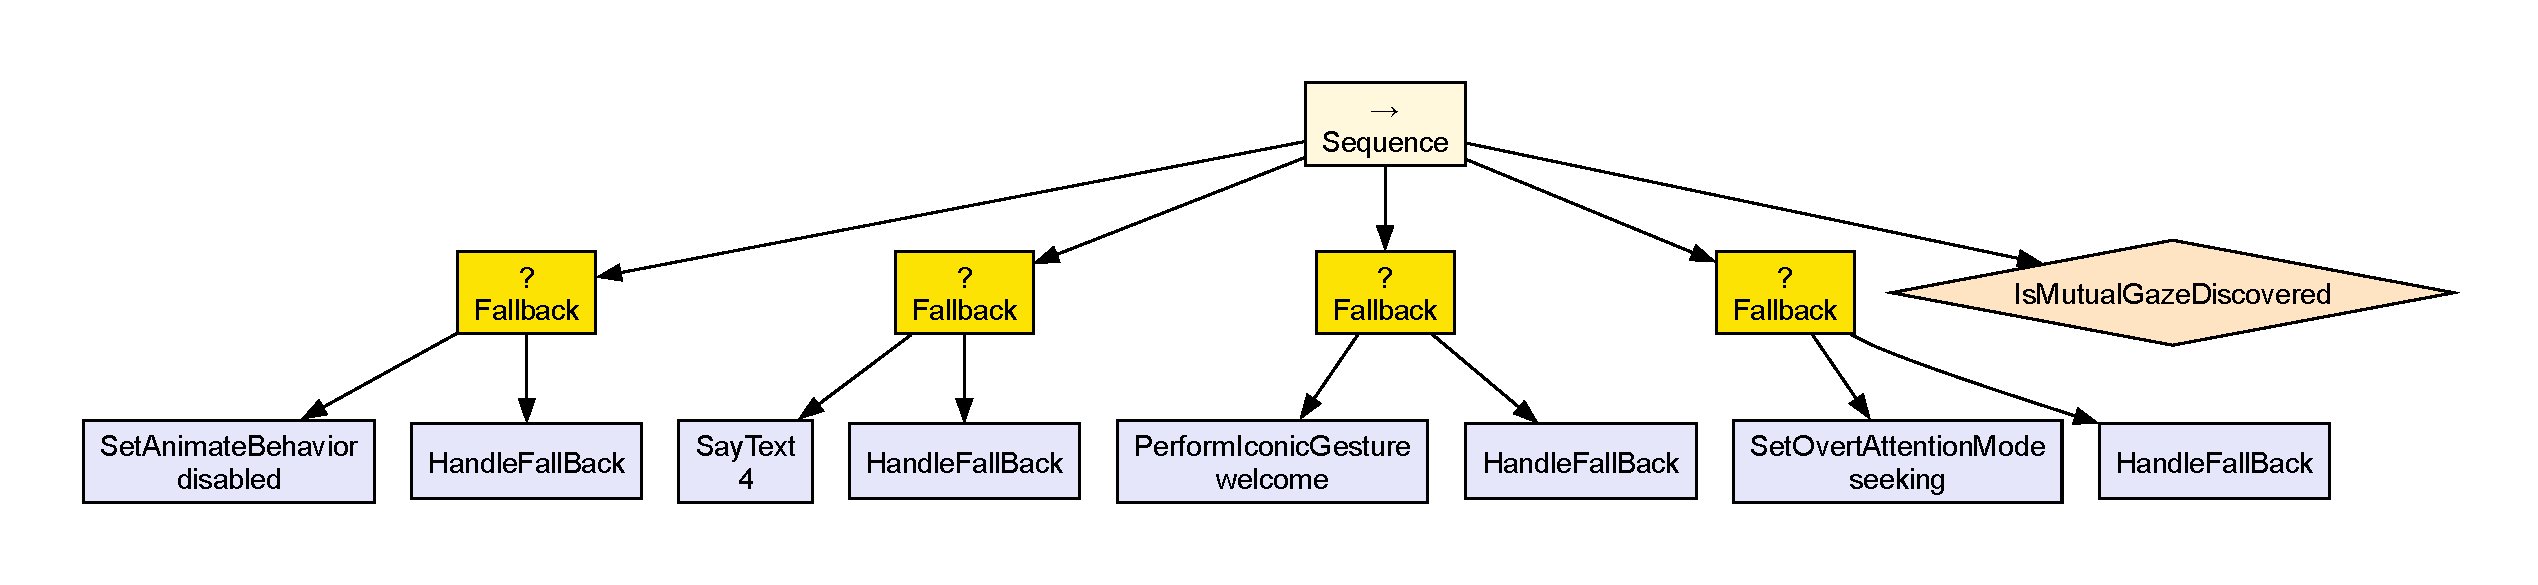
\includegraphics[width=1.1\linewidth]{./diagrams/engage.pdf}
  \caption{Behavior Tree Diagram of the ``EngageVisitor'' Subtree}
  \label{fig:engage_diagram}
\end{figure}
\end{landscape}

%XML representation
\begin{lstlisting}[
  style=XMLStyle, 
  language=XMLCustom, 
  caption={XML Representation of the ``EngageVisitor'' Subtree},
  label={lst:engage_xml}
]
  <BehaviorTree ID="EngageVisitor">
    <Sequence>
      <Fallback>
        <SetAnimateBehavior name="disabled"/>
        <HandleFallBack/>
      </Fallback>
      <Fallback>
        <SayText name="4"
                 _description="Welcome speech"/>
        <HandleFallBack/>
      </Fallback>
      <Fallback>
        <PerformIconicGesture name="welcome"/>
        <HandleFallBack/>
      </Fallback>
      <Fallback>
        <SetOvertAttentionMode name="seeking"/>
        <HandleFallBack/>
      </Fallback>
      <IsMutualGazeDiscovered/>
    </Sequence>
  </BehaviorTree>
\end{lstlisting}



\newpage

\subsubsection{QueryVisitorResponse Subtree}
%- - - - - - - - - - - - - - - - - - - - -} 
 
After the initial greeting, the robot seeks confirmation from the visitor about whether they would like to take the tour. This segment handles both speech-based and tablet-based responses. The robot asks a clear question, and waits a certain amount of time for an ``affirmative'' response (using either automatic speech recognition or a visual touch interface as input). If the response is positive, the robot proceeds to the next segment. Otherwise, it provides a polite response and ends the interaction.

% Tree diagram
\begin{landscape}

\hspace{-2cm}
\begin{figure}[H]
  \centering
  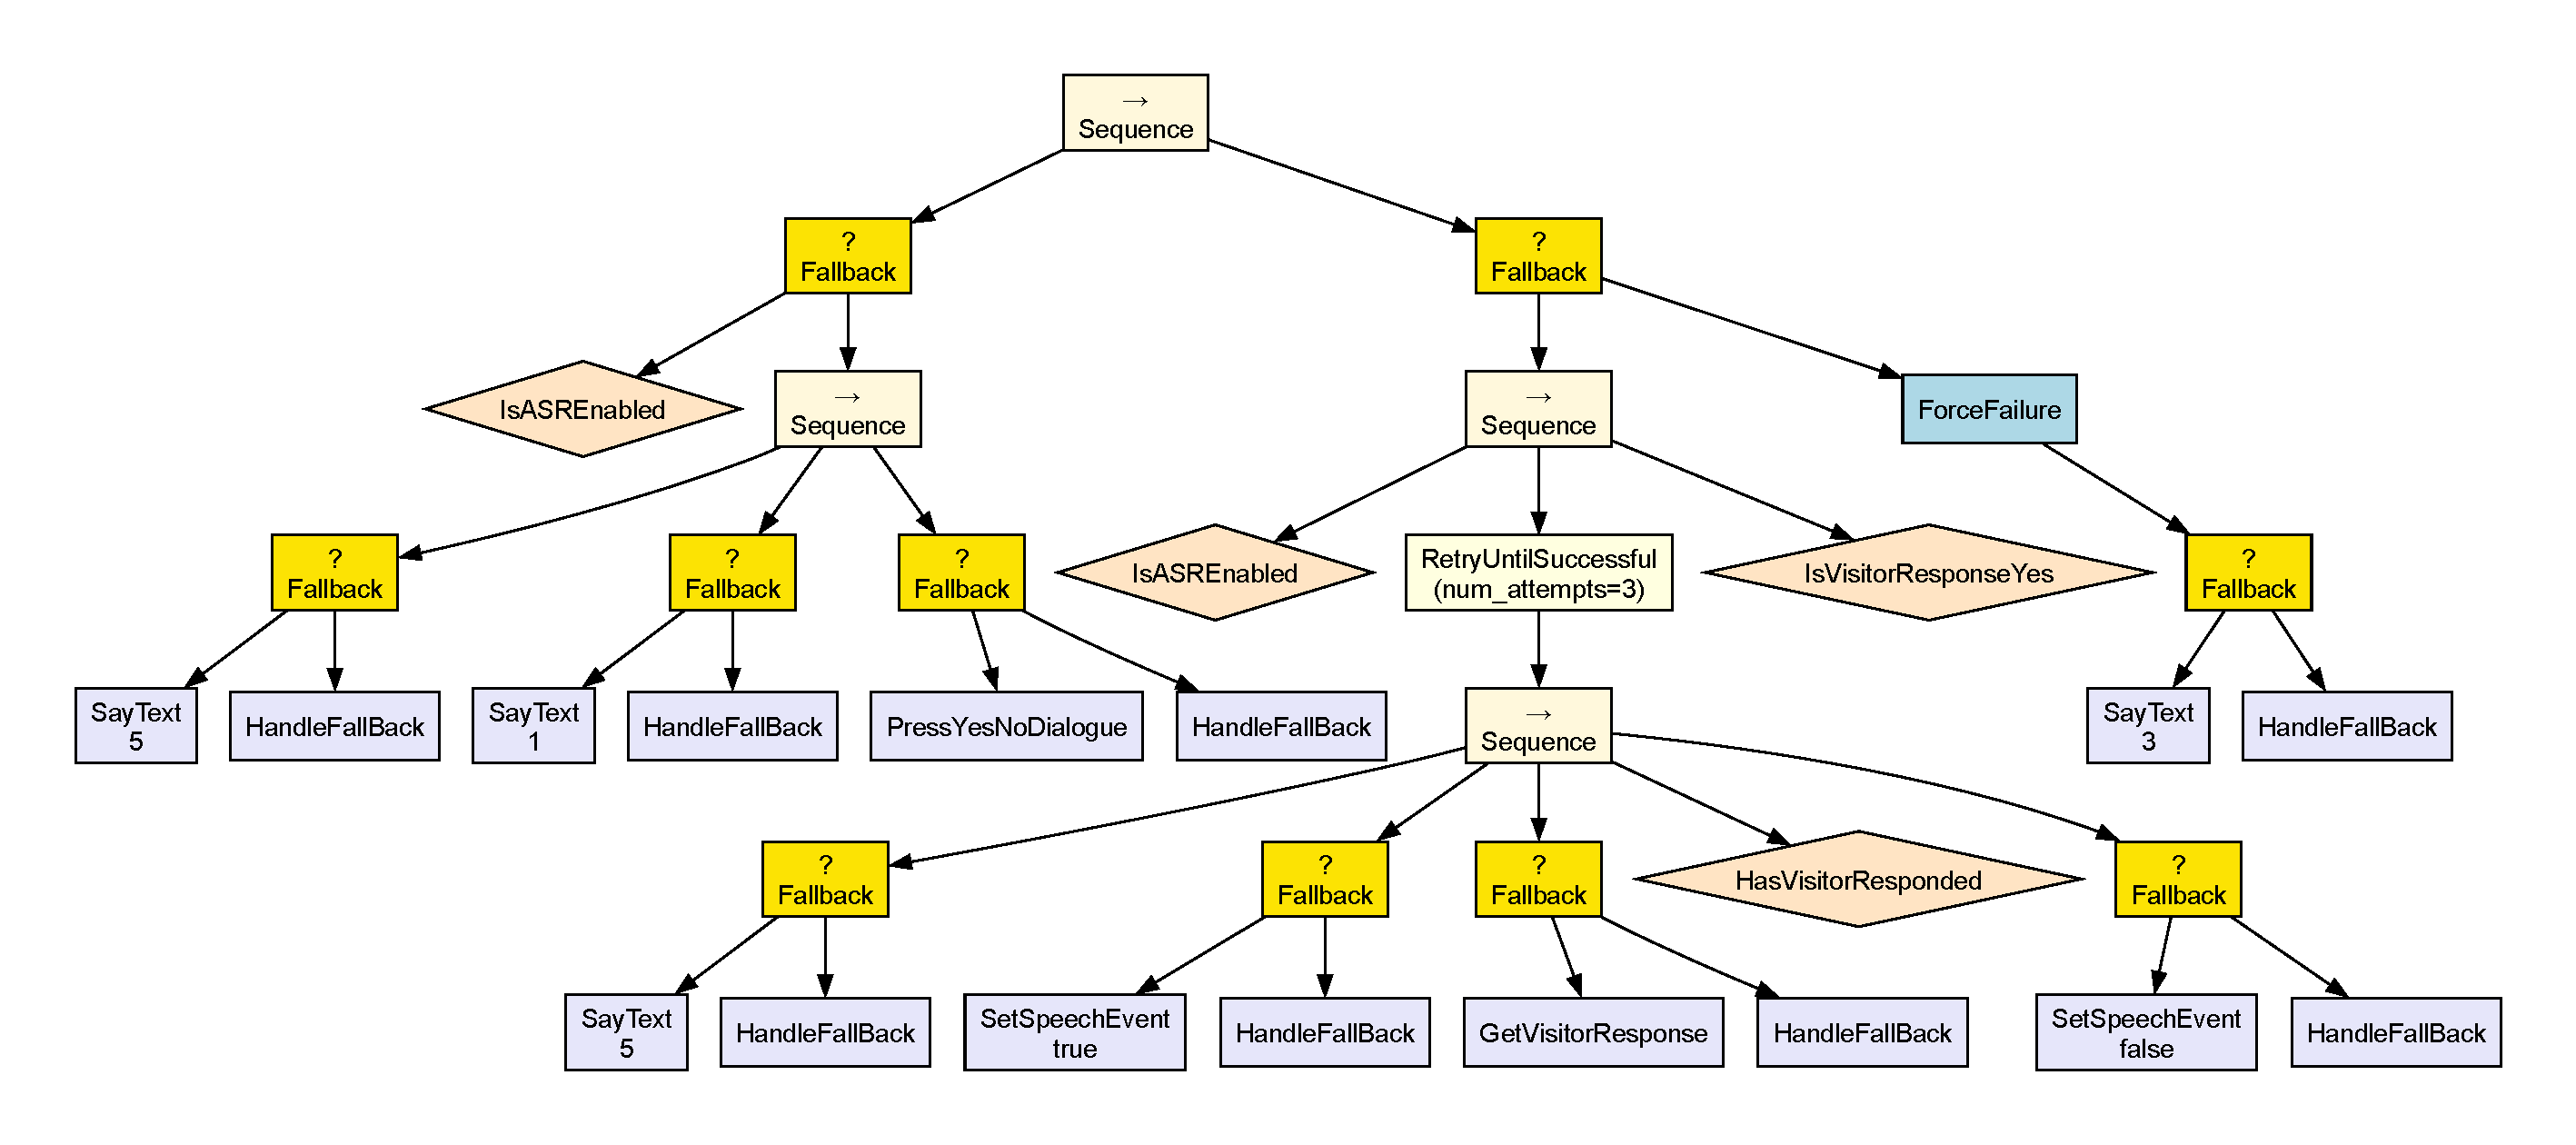
\includegraphics[width=1.08\linewidth]{./diagrams/query.pdf}
  \caption{Behavior Tree Diagram of the ``QueryVisitorResponse'' Subtree}
  \label{fig:query_diagram}
\end{figure}
\end{landscape}

%XML representation
\begin{lstlisting}[
  style=XMLStyle, 
  language=XMLCustom, 
  caption={XML Representation of the ``QueryVisitorResponse'' Subtree},
  label={lst:query_xml}
]
<BehaviorTree ID="QueryVisitorResponse">
    <Sequence>
      <Fallback>
        <IsASREnabled/>
        <Sequence>
          <Fallback>
            <SayText name="5"
                     _description="Query Tour Speech"/>
            <HandleFallBack/>
          </Fallback>
          <Fallback>
            <SayText name="1"
                     _description="Press &quot;yes&quot; or &quot;no&quot; speech"/>
            <HandleFallBack/>
          </Fallback>
          <Fallback>
            <PressYesNoDialogue/>
            <HandleFallBack/>
          </Fallback>
        </Sequence>
      </Fallback>
      <Fallback>
        <Sequence>
          <IsASREnabled/>
          <RetryUntilSuccessful num_attempts="3">
            <Sequence>
              <Fallback>
                <SayText name="5"
                         _description="Query Tour Speech"/>
                <HandleFallBack/>
              </Fallback>
              <SetSpeechEvent name="true"/>
              <Sequence>
                <Delay delay_msec="2000">
                  <Fallback>
                    <GetVisitorResponse/>
                    <HandleFallBack/>
                  </Fallback>
                </Delay>
              </Sequence>
              <HasVisitorResponded/>
              <SetSpeechEvent name="false"/>
            </Sequence>
          </RetryUntilSuccessful>
          <IsVisitorResponseYes/>
        </Sequence>
        <ForceFailure>
          <Fallback>
            <SayText name="3"
                     _description="Maybe another time speech"/>
            <HandleFallBack/>
          </Fallback>
        </ForceFailure>
      </Fallback>
    </Sequence>
\end{lstlisting}

 
\newpage

\subsubsection{VisitExhibit Subtree}
%- - - - - - - - - - - - - - - - - - - - -} 
 
With a positive response, the tour moves into the exhibit visit segment. Here, the robot guides the visitor from one exhibit to another. For each exhibit, the robot retrieves and announces information about the exhibit from a knowledge base, navigates to the location, checks for visual contact to verify continuation, uses gestures such as pointing to highlight key aspects of the exhibit, and provides descriptive commentary about what is being shown. The core part of this subtree is designed to be repeatable for each exhibit along the tour route. Once all exhibits have been visited, the robot navigates to tis ``Home'' location, communicates that the tour has ended, expresses gratitude and hope that the visitor enjoyed the tour.
% Tree diagram
\begin{landscape}
  \setlength{\topmargin}{-1.5cm}
  \setlength{\footskip}{4cm}  
  \vspace{3cm}
  \begin{figure}[H]
    \hspace{-3.55cm} % Move the figure to the left
    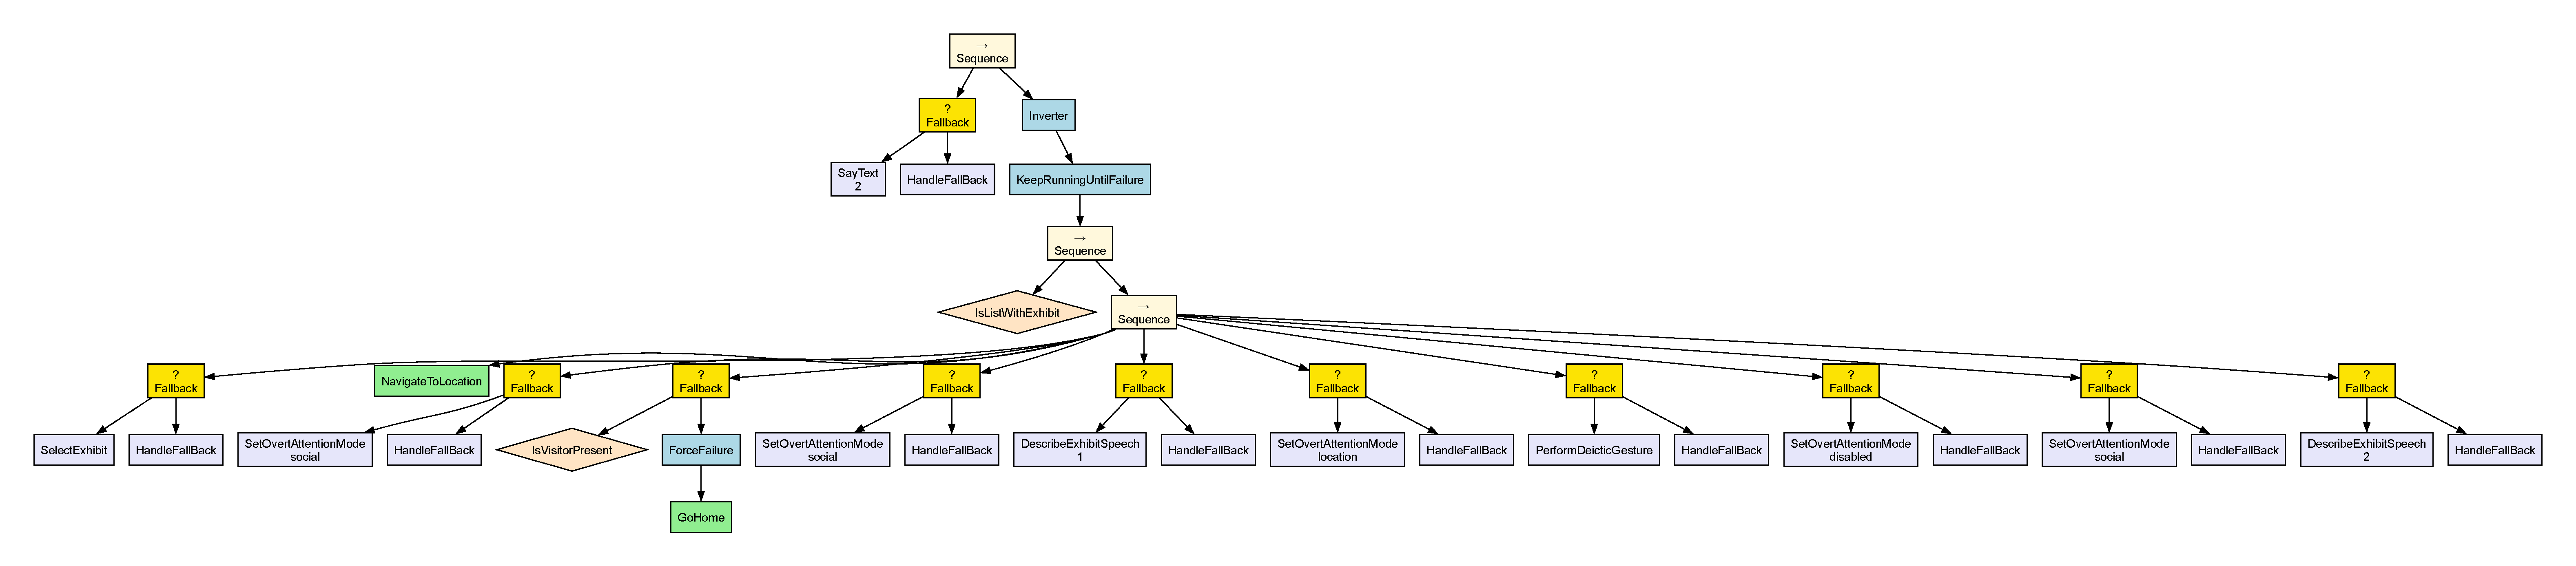
\includegraphics[width=1.25\linewidth]{./diagrams/visit.pdf}
    \caption{Behavior Tree Diagram of the ``VisitExhibit'' Subtree}
    \label{fig:visit_diagram}
  \end{figure}
\end{landscape}


%XML representation
\begin{lstlisting}[
  style=XMLStyle, 
  language=XMLCustom, 
  caption={XML Representation of the ``VisitExhibit'' Subtree},
  label={lst:visit_xml}
]

  <BehaviorTree ID="VisitExhibit">
    <Sequence>
      <Fallback>
        <SayText name="2"
                 _description="Follow me speech"/>
        <HandleFallBack/>
      </Fallback>
      <Inverter>
        <KeepRunningUntilFailure>
          <Sequence>
            <IsListWithExhibit/>
            <Sequence>
              <Fallback>
                <SelectExhibit/>
                <HandleFallBack/>
              </Fallback>
              <SubTree ID="NavigateToLocation"/>
              <Fallback>
                <SetOvertAttentionMode name="social"/>
                <HandleFallBack/>
              </Fallback>
              <Fallback>
                <IsVisitorPresent/>
                <ForceFailure>
                  <SubTree ID="GoHome"/>
                </ForceFailure>
              </Fallback>
              <Fallback>
                <DescribeExhibitSpeech name="1"/>
                <HandleFallBack/>
              </Fallback>
              <Fallback>
                <SetOvertAttentionMode name="location"/>
                <HandleFallBack/>
              </Fallback>
              <Fallback>
                <PerformDeicticGesture/>
                <HandleFallBack/>
              </Fallback>
              <Fallback>
                <SetOvertAttentionMode name="disabled"/>
                <HandleFallBack/>
              </Fallback>
              <Fallback>
                <SetOvertAttentionMode name="social"/>
                <HandleFallBack/>
              </Fallback>
              <Fallback>
                <DescribeExhibitSpeech name="2"/>
                <HandleFallBack/>
              </Fallback>
            </Sequence>
          </Sequence>
        </KeepRunningUntilFailure>
      </Inverter>
    </Sequence>
  </BehaviorTree>
\end{lstlisting}
 
\subsubsection{EndTour Subtree}
%- - - - - - - - - - - - - - - - - - - - -} 
 
The final segment concludes the tour experience. Once all the exhibits have been visited and the robot has navigated back to its ``Home'' location, it finally says goodbye while performing a farewell gesture. This segment ensures a polite and complete wrap-up of the interaction.

% Tree diagram
\begin{figure}[H]
  \centering
  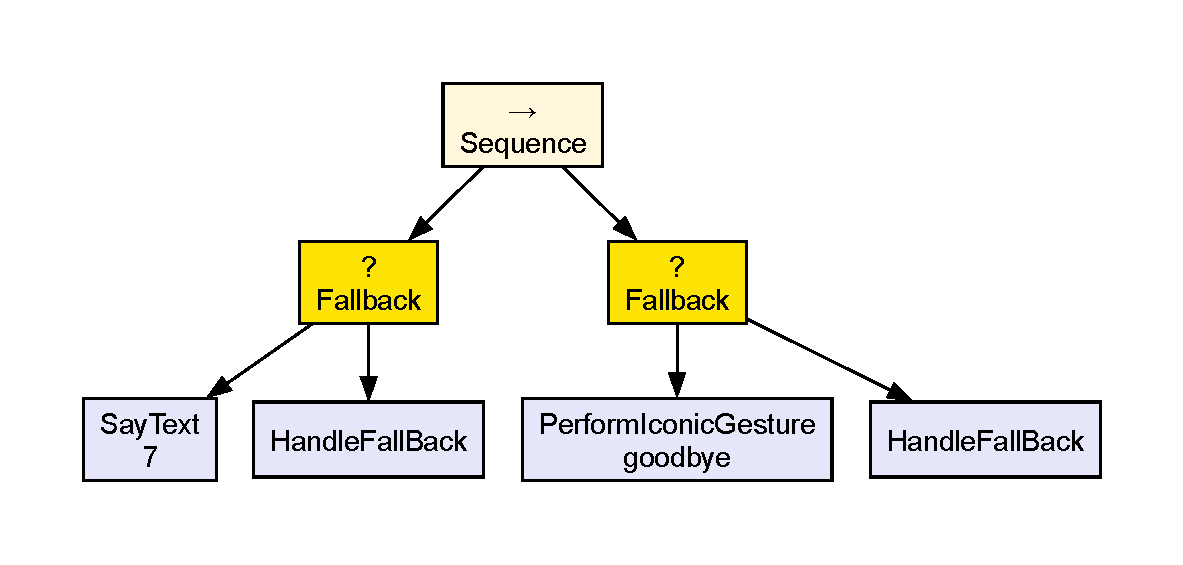
\includegraphics[width=0.7\textwidth]{./diagrams/end.pdf}
  \caption{Behavior Tree Diagram of the ``EndTour'' Subtree}
  \label{fig:end_diagram}
\end{figure}
\bigskip

%XML representation
\begin{lstlisting}[
  style=XMLStyle, 
  language=XMLCustom, 
  caption={XML Representation of the ``EndTour'' Subtree},
  label={lst:end_xml}
]
  <BehaviorTree ID="EndTour">
  <Sequence>
    <Fallback>
      <SayText name="7" _description="Say Goodbye speech"/>
      <HandleFallBack/>
    </Fallback>
    <Fallback>
      <PerformIconicGesture name="goodbye"/>
      <HandleFallBack/>
    </Fallback>
  </Sequence>
</BehaviorTree>
\end{lstlisting}

\subsubsection{NavigateToLocation Subtree}
\label{section:navigate_to_location}
%- - - - - - - - - - - - - - - - - - - - - - - - -} 

The \texttt{NavigateToLocation} encapsulates a sequence of behaviors that are executed whenever the robot performs a navigation task. The main mission node in this subtree is the \textbf{Navigate} action node. This node is the one that's directly responsible for navigating the robot to a specified location. The robot uses its localization and mapping capabilities to plan a path to the target location and execute the navigation.
But, before the robot navigates to a location, it must first disable \textbf{overt attention mode}. This is necessary since the robot doesn't need to set its gaze anywhere but right in front of it. The robot must focus on the navigation task and ensure it reaches the target location successfully.
\begin{figure}[H]
  \centering
  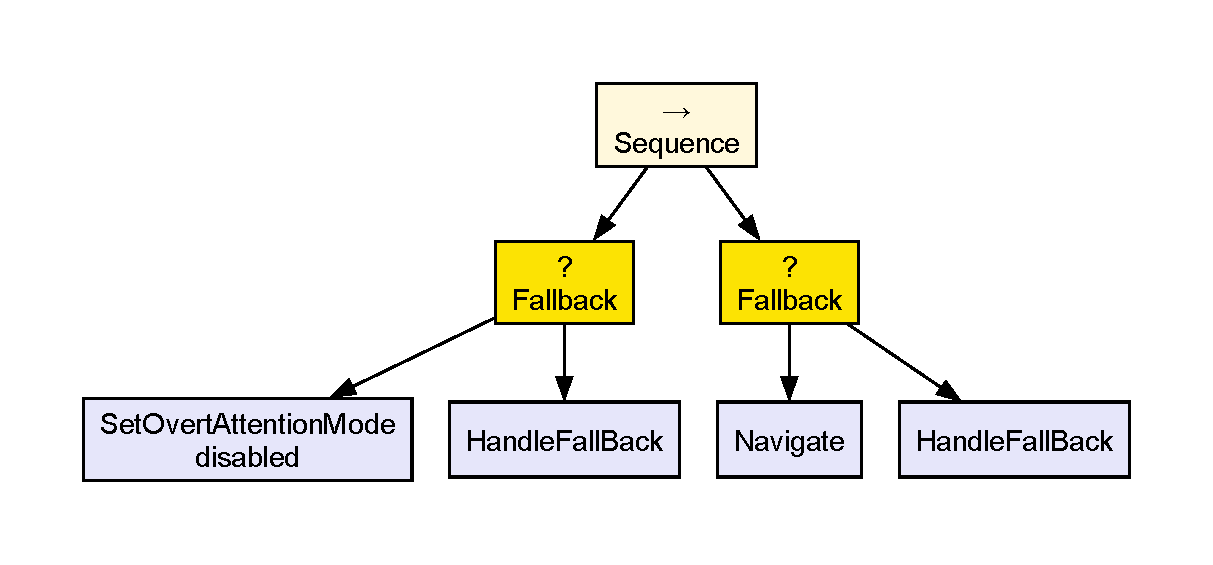
\includegraphics[width=0.7\textwidth]{./diagrams/navigate.pdf}
  \caption{Behavior Tree Diagram of the ``NavigateToLocation'' Subtree}
  \label{fig:navigate_diagram}
\end{figure}

\bigskip
\bigskip

\begin{lstlisting}[
  style=XMLStyle, 
  language=XMLCustom, 
  caption={XML Representation of the ``NavigateToLocation'' Subtree},
  label={lst:navigate_xml}
]
  <BehaviorTree ID="NavigateToLocation">
  <Sequence>
    <Fallback>
      <SetOvertAttentionMode name="disabled"/>
      <HandleFallBack/>
    </Fallback>
    <Fallback>
      <Navigate/>
      <HandleFallBack/>
    </Fallback>
  </Sequence>
</BehaviorTree>
\end{lstlisting}

\subsubsection{GoHome Subtree}
%- - - - - - - - - - - - - - - - - - - - - - - - -} 
 
The \texttt{GoHome} subtree encapsulates a set of behaviors that are consistently executed whenever the robot is required to return to its designated ``Home'' location. This location corresponds to the point where the robot initially began the tour. The process begins with the \texttt{RetrieveInitialLocation} action node, which retrieves the coordinates of the ``Home'' location. Subsequently, the robot invokes the \texttt{NavigateToLocation} subtree to execute the navigation behavior. The implementation details of the navigation logic can be found in Section~\ref{section:navigate_to_location}.

% Tree diagram
\begin{figure}[H]
  \centering
  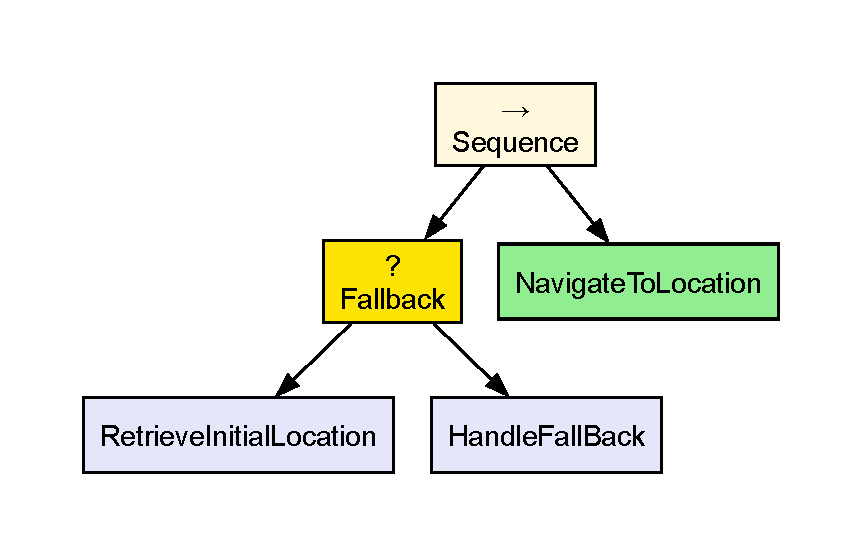
\includegraphics[width=0.7\textwidth]{./diagrams/gohome.pdf}
  \caption{Behavior Tree Diagram of the ``GoHome'' Subtree}
  \label{fig:gohome_diagram}
\end{figure}
%XML representation
\begin{lstlisting}[
  style=XMLStyle, 
  language=XMLCustom, 
  caption={XML Representation of the ``GoHome'' Subtree},
  label={lst:gohome_xml}
]
<BehaviorTree ID="GoHome">
  <Sequence>
    <Fallback>
      <RetrieveInitialLocation/>
      <HandleFallBack/>
    </Fallback>
    <SubTree ID="NavigateToLocation"/>
  </Sequence>
</BehaviorTree>

\end{lstlisting}


\subsection{Mission Nodes}
%-------------------------
\label{section:mission_nodes}

The leaf nodes, which include both action and condition nodes, are where the custom functionality is implemented. Combined with control flow nodes, these building blocks enable the definition of the desired behaviors. A total of 21 action and condition nodes were defined for the ``Lab Tour'' scenario, with many of these nodes reused multiple times throughout the behavior tree. These custom nodes are comprehensively listed in Table \ref{tab:implemented_mission_nodes}, which provides the name, type, and description of each node. Note that the actual logic and implementation of these nodes are not detailed here; they are encapsulated within the robot mission interpreter, which executes the behavior tree, as described in Deliverable D5.4.3 Robot Mission Interpreter.


\begin{longtable}[c]{|p{4.65cm}|p{1.4cm}|p{7.4cm}|}
  \caption{High-Level Mission Node Descriptions} \label{tab:implemented_mission_nodes_custom}\\

  \hline
  \rowcolor{gray!30}
  \small{\textbf{Node}} & \small{\textbf{Type}} & \small{\textbf{Description}} \\ \hline
  \endfirsthead
  \hline
  \rowcolor{gray!30}
  \small{\textbf{Node}} & \small{\textbf{Type}} & \small{\textbf{Description}} \\ \hline
  \endhead

  \small{\texttt{DescribeExhibitSpeech}} & \small{Action} & \small{Delivers an auditory description of the selected exhibit to inform and engage the visitor.} \\ \hline
  \small{\texttt{GetVisitorResponse}} & \small{Action} & \small{Captures and processes a response from the visitor, used after a prompt or question.} \\ \hline
  \small{\texttt{HandleFallBack}} & \small{Action} & \small{Handles unexpected states or errors by triggering fallback mechanisms in the mission logic.} \\ \hline
  \small{\texttt{HasVisitorResponded}} & \small{Condition} & \small{Checks if a visitor has provided a response or not.} \\ \hline
  \small{\texttt{IsASREnabled}} & \small{Condition} & \small{Checks whether the automatic speech recognition (ASR) system is enabled and operational.} \\ \hline
  \small{\texttt{IsListWithExhibit}} & \small{Condition} & \small{Determines whether there is an available list of exhibits to present or navigate to.} \\ \hline
  \small{\texttt{IsMutualGazeDiscovered}} & \small{Condition} & \small{Detects whether mutual gaze between the robot and the visitor has been established.} \\ \hline
  \small{\texttt{IsVisitorDiscovered}} & \small{Condition} & \small{Checks if a visitor is currently detected within the interaction range of the robot.} \\ \hline
  \small{\texttt{IsVisitorResponseYes}} & \small{Condition} & \small{Determines whether the visitor has provided an affirmative response to a previous query.} \\ \hline
  \small{\texttt{Navigate}} & \small{Action} & \small{Directs the robot to move toward a specified target location.} \\ \hline
  \small{\texttt{PerformDeicticGesture}} & \small{Action} & \small{Performs a pointing gesture to draw the visitor’s attention to a specific area or exhibit.} \\ \hline
  \small{\texttt{PerformIconicGesture}} & \small{Action} & \small{Executes a recognizable gesture such as a goodbye wave or a welcome motion to visually complement the interaction.} \\ \hline
  \small{\texttt{PressYesNoDialogue}} & \small{Action} & \small{Initiates a Yes/No interaction via buttons or a GUI to capture explicit visitor responses.} \\ \hline
  \small{\texttt{RetrieveInitialLocation}} & \small{Action} & \small{Retrieves the robot's starting location.} \\ \hline
  \small{\texttt{RetrieveListOfExhibits}} & \small{Action} & \small{Collects and stores the list of exhibits that will be part of the guided tour.} \\ \hline
  \small{\texttt{SayText}} & \small{Action} & \small{Enables the robot to vocalize a given text string.} \\ \hline
  \small{\texttt{SelectExhibit}} & \small{Action} & \small{Chooses the next exhibit from the list retrieved using ``RetrieveListOfExhibits''} \\ \hline
  \small{\texttt{SetAnimateBehavior}} & \small{Action} & \small{Sets the state of the animation behaviors to enhance the robot’s lifelike presence.} \\ \hline
  \small{\texttt{SetOvertAttentionMode}} & \small{Action} & \small{Sets the robot’s overt attention mode, influencing how it visually engages with its environment.} \\ \hline
  \small{\texttt{SetRobotPose}} & \small{Action} & \small{Assigns a specific pose or position to the robot in the environment.} \\ \hline
  \small{\texttt{SetSpeechEvent}} & \small{Action} & \small{Activates or deactivates the automatic speech recognition feature.} \\ \hline
  \small{\texttt{StartOfTree}} & \small{Action} & \small{Used for debugging and initializing mission wide variables.} \\ \hline

\end{longtable}




%%\newpage
\bibliographystyle{unsrt}
%================================================================
\bibliography{cognitive_systems.bib}               
\addcontentsline{toc}{section}{References}

 

\pagebreak
\section*{Principal Contributors}
%===============================================================
\label{contributors}
\addcontentsline{toc}{section}{Principal Contributors}
The main authors of this deliverable are as follows (in alphabetical order).
\blank
~
\blank
Tsegezeab Tefferi, Carnegie Mellon University Africa.\\   
David Vernon, Carnegie Mellon University Africa.\\   
  

\newpage
\section*{Document History}
%================================================================
\addcontentsline{toc}{section}{Document History}
\label{document_history}

\begin{description}

\item [Version 1.0]~\\
First version created by moving and reorganizing Section 3 from Deliverable D5.4.2. \\
David Vernon.\\
18 April 2025.   \\               

\item [Version 1.1]~\\
Updated the list of high-level mission nodes, along with their descriptions to reflect the simplified mission specification.\\
Updated the XML output of the mission specification and revised the descriptions of each subtree to reflect the new behavior tree structure.\\
Replaced the large, comprehensive behavior tree diagram with individual diagrams for each subtree\\
Resolved various issues noted in the previous version.\\
Tsegazeab Tefferi.\\
05 May 2025

\item [Version 1.2]~\\
Updated the XML outputs, the diagrams and the list of high-level mission nodes to reflect the current version of the behavior tree.\\
Updated the diagrams to be centered and to fit within the page margins.\\
Revised the description of the mission specification to clarify that it is not an exact replication of the scenario outlined in D2.1, but rather a functional implementation.
Tsegazeab Tefferi.\\
01 June 2025

\end{description}


\end{document}
